\documentclass[journal,12pt,twocolumn]{IEEEtran}

\usepackage{setspace}
\usepackage{gensymb}
\singlespacing
\usepackage[cmex10]{amsmath}

\usepackage{amsthm}

\usepackage{mathrsfs}
\usepackage{txfonts}
\usepackage{stfloats}
\usepackage{bm}
\usepackage{cite}
\usepackage{cases}
\usepackage{subfig}

\usepackage{longtable}
\usepackage{multirow}

\usepackage{enumitem}
\usepackage{mathtools}
\usepackage{steinmetz}
\usepackage{tikz}
\usepackage{circuitikz}
\usepackage{verbatim}
\usepackage{tfrupee}
\usepackage[breaklinks=true]{hyperref}
\usepackage{graphicx}
\usepackage{tkz-euclide}

\usetikzlibrary{calc,math}
\usepackage{listings}
    \usepackage{color}                                            %%
    \usepackage{array}                                            %%
    \usepackage{longtable}                                        %%
    \usepackage{calc}                                             %%
    \usepackage{multirow}                                         %%
    \usepackage{hhline}                                           %%
    \usepackage{ifthen}                                           %%
    \usepackage{lscape}     
\usepackage{multicol}
\usepackage{chngcntr}

\DeclareMathOperator*{\Res}{Res}

\renewcommand\thesection{\arabic{section}}
\renewcommand\thesubsection{\thesection.\arabic{subsection}}
\renewcommand\thesubsubsection{\thesubsection.\arabic{subsubsection}}

\renewcommand\thesectiondis{\arabic{section}}
\renewcommand\thesubsectiondis{\thesectiondis.\arabic{subsection}}
\renewcommand\thesubsubsectiondis{\thesubsectiondis.\arabic{subsubsection}}


\hyphenation{op-tical net-works semi-conduc-tor}
\def\inputGnumericTable{}                                 %%

\lstset{
%language=C,
frame=single, 
breaklines=true,
columns=fullflexible
}
\begin{document}

\newcommand{\BEQA}{\begin{eqnarray}}
\newcommand{\EEQA}{\end{eqnarray}}
\newcommand{\define}{\stackrel{\triangle}{=}}
\bibliographystyle{IEEEtran}
\raggedbottom
\setlength{\parindent}{0pt}
\providecommand{\mbf}{\mathbf}
\providecommand{\pr}[1]{\ensuremath{\Pr\left(#1\right)}}
\providecommand{\qfunc}[1]{\ensuremath{Q\left(#1\right)}}
\providecommand{\sbrak}[1]{\ensuremath{{}\left[#1\right]}}
\providecommand{\lsbrak}[1]{\ensuremath{{}\left[#1\right.}}
\providecommand{\rsbrak}[1]{\ensuremath{{}\left.#1\right]}}
\providecommand{\brak}[1]{\ensuremath{\left(#1\right)}}
\providecommand{\lbrak}[1]{\ensuremath{\left(#1\right.}}
\providecommand{\rbrak}[1]{\ensuremath{\left.#1\right)}}
\providecommand{\cbrak}[1]{\ensuremath{\left\{#1\right\}}}
\providecommand{\lcbrak}[1]{\ensuremath{\left\{#1\right.}}
\providecommand{\rcbrak}[1]{\ensuremath{\left.#1\right\}}}
\theoremstyle{remark}
\newtheorem{rem}{Remark}
\newcommand{\sgn}{\mathop{\mathrm{sgn}}}
\providecommand{\abs}[1]{\vert#1\vert}
\providecommand{\res}[1]{\Res\displaylimits_{#1}} 
\providecommand{\norm}[1]{\lVert#1\rVert}
%\providecommand{\norm}[1]{\lVert#1\rVert}
\providecommand{\mtx}[1]{\mathbf{#1}}
\providecommand{\mean}[1]{E[ #1 ]}
\providecommand{\fourier}{\overset{\mathcal{F}}{ \rightleftharpoons}}
%\providecommand{\hilbert}{\overset{\mathcal{H}}{ \rightleftharpoons}}
\providecommand{\system}{\overset{\mathcal{H}}{ \longleftrightarrow}}
	%\newcommand{\solution}[2]{\textbf{Solution:}{#1}}
\newcommand{\solution}{\noindent \textbf{Solution: }}
\newcommand{\cosec}{\,\text{cosec}\,}
\providecommand{\dec}[2]{\ensuremath{\overset{#1}{\underset{#2}{\gtrless}}}}
\newcommand{\myvec}[1]{\ensuremath{\begin{pmatrix}#1\end{pmatrix}}}
\newcommand{\mydet}[1]{\ensuremath{\begin{vmatrix}#1\end{vmatrix}}}
\numberwithin{equation}{subsection}
\makeatletter
\@addtoreset{figure}{problem}
\makeatother
\let\StandardTheFigure\thefigure
\let\vec\mathbf
\renewcommand{\thefigure}{\theproblem}
\def\putbox#1#2#3{\makebox[0in][l]{\makebox[#1][l]{}\raisebox{\baselineskip}[0in][0in]{\raisebox{#2}[0in][0in]{#3}}}}
     \def\rightbox#1{\makebox[0in][r]{#1}}
     \def\centbox#1{\makebox[0in]{#1}}
     \def\topbox#1{\raisebox{-\baselineskip}[0in][0in]{#1}}
     \def\midbox#1{\raisebox{-0.5\baselineskip}[0in][0in]{#1}}
\vspace{3cm}
\title{Assignment 3}
\author{Dontha Aarthi - CS20BTECH11015}
\maketitle
\newpage
\bigskip
\renewcommand{\thefigure}{\theenumi}
\renewcommand{\thetable}{\theenumi}
Download all python codes from 
\begin{lstlisting}
    https://github.com/Dontha-Aarthi/AI1103/tree/main/Assignment3/Codes
\end{lstlisting}
and latex-tikz codes from 
\begin{lstlisting}
https://github.com/Dontha-Aarthi/AI1103/blob/main/Assignment3/main.tex
\end{lstlisting}
\section{Problem}
\begin{center}
	(GATE 2019-XE Q.no 1 (Page Number:4)
\end{center}
Let $X$ be the Poisson random variable with parameter $\lambda$ = 1. Then, the probability 
$\pr{2 \leq X \leq 4}$ equals ............
\section{solution}
Let 
\begin{align}
	X\in \{0,1,2,3,4,5...\}
\end{align}
We know that, for a poisson random variable $X$ with a given parameter $\lambda$, probability of $X=k$ is:
\begin{align} \label{eq_0}
	\pr{X=k}=\left(\frac{\lambda^k e^{-\lambda}}{k!}\right)	
\end{align}
First, lets calculate the PMF of the distribution by plugging the values of $k$ into \ref{eq_0},
\begin{table}[ht]
  \centering
  \begin{tabular}{|c|c|c|c|c|c|}
    \hline
    k &  0 & 1 & 2 & 3 & 4\\
    \hline
    $\pr{X=k}$ & 1/e & 1/e & 1/2e & 1/6e & 1/24e\\
    \hline
\end{tabular}
\caption{ PMF}
\label{Table_0}
\end{table}\\
The CDF is as follows:
\begin{table}[ht]
  \centering
  \begin{tabular}{|c|c|c|c|c|c|}
    \hline
    x &  0 & 1 & 2 & 3 & 4\\
    \hline
    $F(x)$ & 1/e & 2/e & 5/2e & 8/3e & 65/24e\\
    \hline
\end{tabular} 
\caption{CDF}
\label{Table_1}
\end{table}\\
The graph of CDF is shown below
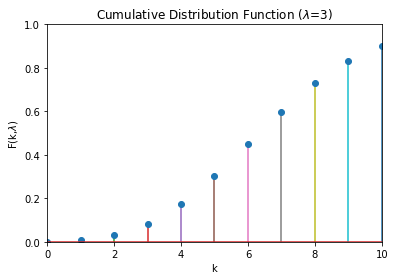
\includegraphics[width=\linewidth]{cdf.png}

And also,
\begin{align}
    \Pr\brak{x < X \le y} = F\brak{y} - F\brak{x}\label{eq_1}
\end{align}

So, now we can find the value of $\pr{2 \leq X \leq 4}$ and also its given that $\lambda$=1.\\
We can represent the value of $\pr{2 \leq X \leq 4}$ as $\pr{1 \le X \leq 4}$.\\

Now by using \ref{eq_1},
\begin{align}
    \pr{2 \leq X \leq 4} 
    & = \pr{1 < X \leq 4}\\
    & = F(4)-F(1)\\
    & = \frac{65}{24e}-\frac{2}{e}\\
    & = \frac{17}{24e}
\end{align}\\

The graph for theoretical result vs simulation is given below\\
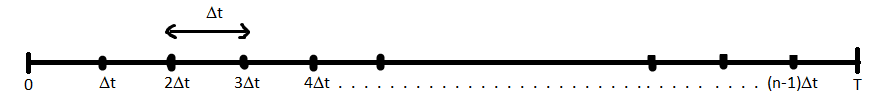
\includegraphics[width=\linewidth]{figure1.png}
 
\end{document}